% Drawn by scripts/revision3/fig_appendix_schematics.py; the .pptx is the
% editable source and is released with the paper.
\begin{figure*}[t]
\centering
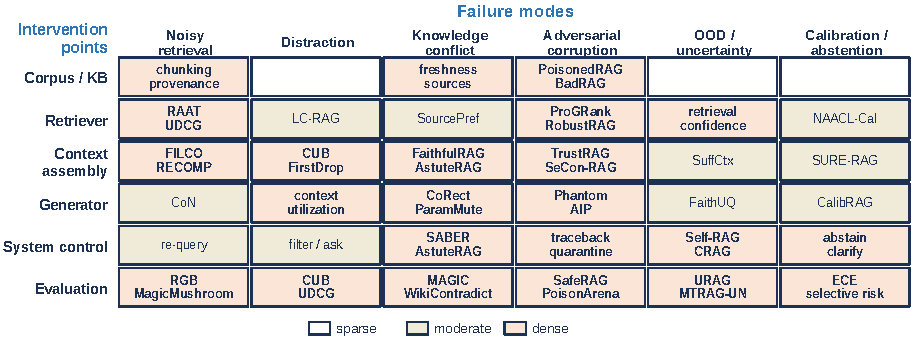
\includegraphics[width=\textwidth]{figures/generated/fig_failure_matrix.pdf}%
\caption{Schematic literature-family $\times$ intervention matrix. Shading and
example labels are illustrative design aids, not counts from Map~B;
quantitative Map-B distributions appear in Table~\ref{tab:corpus-stats}. Rows
are coordinate C3 and columns are coordinate C1, which is why a cell, not a
column, is the unit at which two systems become comparable.}
\label{fig:failure-intervention-matrix}
\end{figure*}
